\documentclass[10pt,compress,handout]{beamer}
    \useoutertheme{miniframes}
    \usepackage[english]{babel}
    %\usepackage[margin=1in]{geometry}

    \usepackage{amsmath}
    \usepackage{amsfonts} 
    \usepackage{amssymb}
    \usepackage{amsthm}
    \usepackage{mathtools}

    \usepackage[utf8]{inputenc}
    %\usepackage[exscale, amsfonts, amssymb]{concmath}
    %\renewcommand*{\bfseries}{\mdseries}

    \usepackage{float}
    \usepackage{graphicx}
    \usepackage{caption}
    \usepackage{subcaption}

    \graphicspath{{./src/figures/}}

    %\usepackage{fancyhdr} %custom headers and footers layout
    \usepackage{lastpage} %package to print the last page
    %\pagestyle{fancy} %fancy page style

    \usepackage{textcomp} 
    \usepackage{multicol} 
    \usepackage{multirow}

    \usepackage[table]{xcolor}
    \usepackage{booktabs}

    \usepackage[backend=biber,
    bibstyle=ieee, 
    citestyle=numeric-comp,
    natbib=true,
    doi=false, 
    url=false,
    isbn=false,
    mincitenames=1,
    maxcitenames=1,
    minbibnames=1,
    maxbibnames=99,
    backref=false,]
    {biblatex}
    \addbibresource[label=main]{./src/references.bib}

    \usepackage{url}
    \usepackage{hyperref}

    %edit the properties of your PDF documents which will be displayed
    \hypersetup{
        bookmarks=true, 		% show bookmarks bar?
        unicode=true,  		% non-Latin characters in Acrobat’s bookmarks
        pdftoolbar=true,        % show Acrobat’s toolbar?
        pdfmenubar=true,        % show Acrobat’s menu?
        pdffitwindow=true,      % page fit to window when opened
        pdftitle={EIS --- Basics},    % title
        pdfauthor={M. Skocic},     % author
        pdfsubject={},   % subject of the document
        pdfnewwindow=true,      % links in new window
        pdfkeywords={}, % list of keywords
        colorlinks=false,       % false: boxed links; true: colored links
        linkcolor=red,          % color of internal links
        citecolor=green,        % color of links to bibliography
        filecolor=magenta,      % color of file links
        urlcolor=cyan           % color of external links
    }

    \usepackage{tikz}
    \usepackage{circuitikz}
    \usetikzlibrary{decorations.pathmorphing,arrows,calc}

    \title{Electrochemical Impedance Spectroscopy}
    \author{M. Skocic, PhD Electrochemistry and Materials}
    \date{\vfill 
\includegraphics[width=0.70\textwidth]{full_bw.png}}   

    \setlength{\parskip}{6pt}
    \newcommand{\coef}{1}

\begin{document}
    \begin{frame}
        \titlepage
    \end{frame}

    \begin{frame}
        \frametitle{Contents}
        \tableofcontents
    \end{frame}
    
\section{Introduction}
    \begin{frame}{Introduction}
        Time domain (incomplete!) \citep{bard2001}:
        \begin{itemize}
            \item Polarisation: $I=f(U)$
            \item Potential step: $\Delta U$, $I(t)$
            \item Zero Resistance Ammeter: $\int j_{gal} \cdot dt$
        \end{itemize}

        Frequency domain \citep{bard2001}:
        \begin{itemize}
            \item Electrochemical Impedance Spectroscopy
        \end{itemize}

        Advantages of EIS \citep{bard2001}:
        \begin{itemize}
            \item Measurement in small perturbations (approximately linear)
            \item Different processes have different time constants
            \item Large frequency range from $\mu Hz$ to $GHz$
        \end{itemize}
    \end{frame}

\section{Basics}
    \begin{frame}{Black Box Approach}
        Assume a black box with terminals .

        One applies a voltage and measures the current response (or vice versa).

        Periodic signal with an angular frequency $\omega = 2\pi f$
        with $0 \le \omega < \infty$:
        \begin{itemize}
            \item Voltage $V(\omega) = V_0 e^{j \omega t}$  
            \item Voltage $I(\omega) = I_0 e^{j \omega t}$  
        \end{itemize}
        
        \begin{columns}
            \centering
            \column{0.3\textwidth}\centering
                \begin{figure}[h]
                    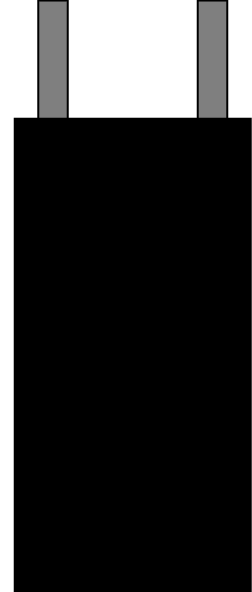
\includegraphics[width=0.5\textwidth]{EIS-black_box}
                \end{figure}
            \column{0.35\textwidth}\centering
                \begin{figure}
                    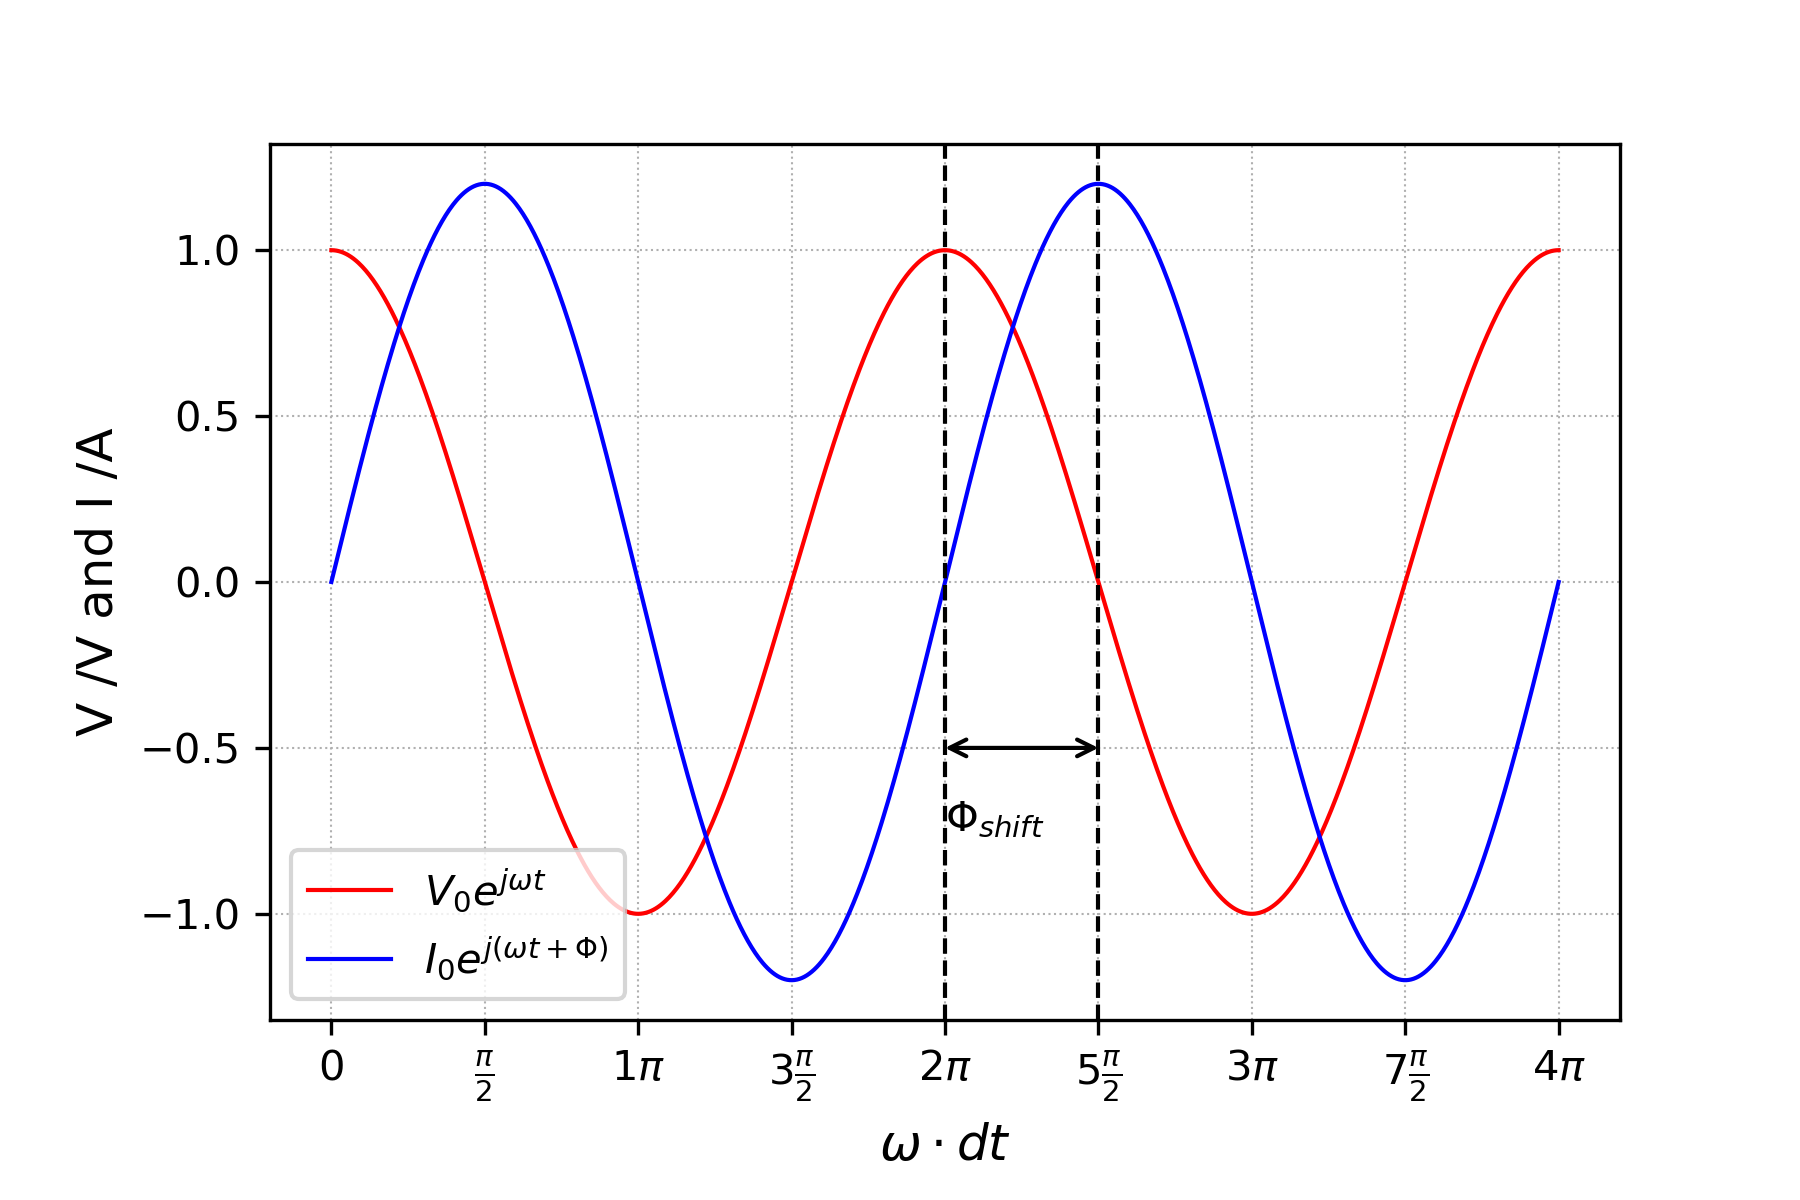
\includegraphics[width=\textwidth]{EIS-ac_waves}
                \end{figure}
            \column{0.35\textwidth}\centering
                \begin{figure}
                    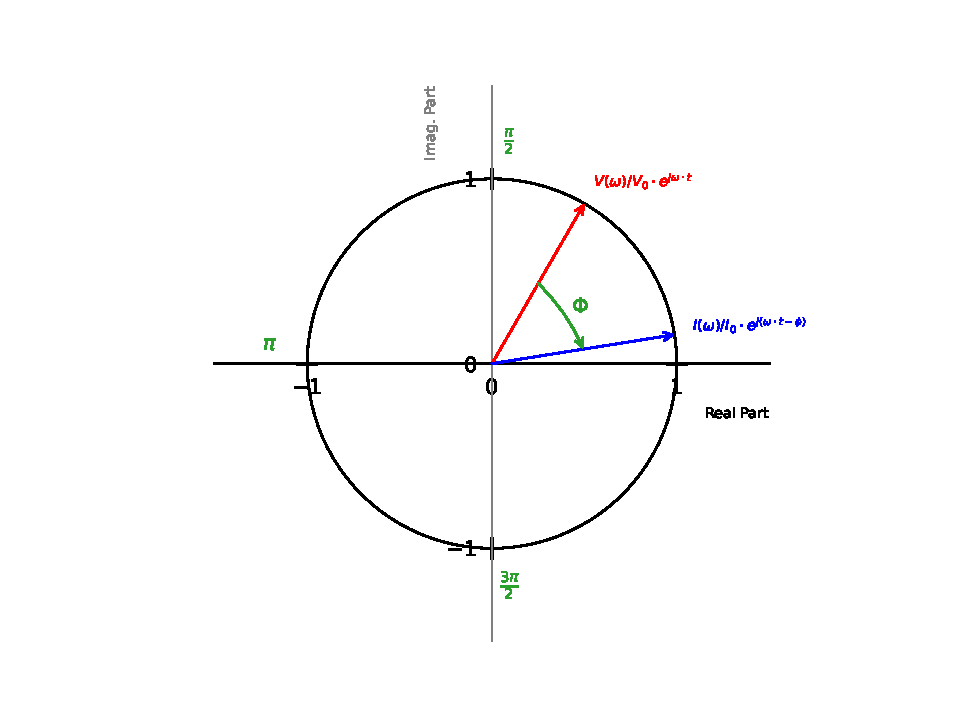
\includegraphics[width=1.3\textwidth]{EIS-ac_waves-trigcircle}
                \end{figure}
        \end{columns}
    \end{frame}
    
    \begin{frame}{What is EIS?}
    a
    \end{frame}


\section{Applications}

% BIBLIOGRAPHY
\begin{frame}[allowframebreaks=0.9]{References}
\AtNextBibliography{\tiny}
%\nocite{*}
\printbibliography
\end{frame}

\end{document}
